% concatenated from main.tex

   \documentclass[final ]{IEEEtran}

% \documentclass[final]{IEEEtran}

%\usepackage{lineno}
%\linenumbers


%\overrideIEEEmargins

 \usepackage{hyperref}  %%%% for clickable links

 \usepackage{datetime}  %% FOR ADDING DATE
\usepackage{nicematrix}
\usepackage{multicol}
\usepackage{mathtools}
\usepackage{url}
\usepackage[makeroom]{cancel}
\usepackage{soul}

\usepackage{amsmath,amssymb}
\usepackage{amsthm,thmtools}
\usepackage{amsfonts}
\usepackage{blkarray}
\usepackage{circuitikz}
\usepackage{bigstrut}
\usepackage{tikz}
\usetikzlibrary{tikzmark,calc,fit}
\usepackage{pgfplots}

 \usepackage{tkz-graph}



%%%\usepackage{theorem}
%\usepackage[dvips]{epsfig}    % ******* for figures ***************
 \usepackage{graphicx}
%\usepackage{auto-pst-pdf}
\usepackage{enumerate}
\usepackage{color}      %******** for colored remarks********

\usepackage{verbatim}

%%\usepackage{refcheck}

%\usepackage{multicol}

\usepackage{amssymb}
\usepackage{amsbsy}
%\usepackage{amsmath}
\usepackage{amsmath,lipsum}
\usepackage{mathabx}
\usepackage{setspace}
\usepackage{url}

%\usepackage{subcaption}
\usepackage{float}
 \usepackage{dsfont}
% \usepackage{cuted} \stripsep-3pt

% \usepackage{caption}
%\captionsetup[table]{skip=10pt}

\iffalse
\usepackage{todonotes}
\newcommand{\rotodo}[1]{\todo[inline]{\textbf{From RO:} #1}}
\fi
%\newcommand{\jjs}[1]{\textcolor{blue}{jjs -- #1}}
\newcommand{\Ave}{\operatorname{Ave}}

\def\Aut{\mathop{\rm Aut}\nolimits}
\def\End{\mathop{\rm End}\nolimits}
\def\Hom{\mathop{\rm Hom}\nolimits}
%\newcommand{\Aut{\operatorname{Aut}}
\def\Lie{\mathop{\rm Lie}\nolimits}
%\newcommand{\Lie}{\operatorname{Lie}}
 \newcommand{\Spec}{\operatorname{Spec}}
 \newcommand{\dist}{\operatorname{dist}}
 \renewcommand{\div}{\operatorname{div}}
 \newcommand{\Int}{\operatorname{int}}
 \newcommand{\Clos}{\operatorname{clos}}
 \newcommand{\real}{\operatorname{Re}}
 \newcommand{\imag}{\operatorname{Im}}
 \newcommand{\diag}{\operatorname{diag}}
 \newcommand{\sign}{\operatorname{sgn}}
 \newcommand{\tr}{\operatorname{tr}}
 \newcommand{\adju}{\operatorname{adj}}
 \newcommand{\suchthat}{\, :  \,}
\newcommand\mycom[2]{\genfrac{}{}{0pt}{}{#1}{#2}}
\newcommand{\spanop}{\operatorname{span}}
\newcommand{\vecop}{\operatorname{vec}}
%%\newcommand{\trace}{\operatorname{trace}}
\newcommand{\inter}{\operatorname{int}}
\newcommand*\diff{\mathop{}\!\mathrm{d}}
\newcommand{\trace}{\operatorname{tr}}
\newcommand\scalemath[2]{\scalebox{#1}

{\mbox{\ensuremath{\displaystyle #2}}}}
%{\theorembodyfont{\rmfamily} \newtheorem{Remark}{Remark}}
%{\theorembodyfont{\rmfamily} \newtheorem{Assumption}{Assumption}}
%%

%\renewcommand{\kbldelim}{(}% Left delimiter
%\renewcommand{\kbrdelim}{)}% Right delimiter

\newcommand{\such}{\, | \,}

%\declaretheorem[name={Example},qed={\lower-0.3ex\hbox{$\square$}} ] {Example}
\newcommand{\ai}{\alpha^i}
\newcommand{\aj}{\alpha^j}
\newcommand{\bi}{\bar{\alpha}^i}
\newcommand{\bj}{\bar{\alpha}^j}
 \newcommand{\sums}{\sum_{l=1}^k\alpha^j_{l}+\alpha^i_{l}}
\newcommand{\U}{U_r^{(1)}}
\newcommand{\sig}[1]{(-1)^{\sum_{l=1}^k#1_l}}
\newcommand{\inR}[1]{\in\R^{#1\times #1}}

%\declaretheorem[name={Definition}  ] {Definition}
\newtheorem{theorem}{Theorem}
\newtheorem{assumption}{Assumption}
\newtheorem{claim}{Claim}
\newtheorem{definition}{Definition}
\newtheorem{proposition}{Proposition}%USE SAME COUNTER AS IN THM
\newtheorem{lemma}{Lemma}%USE SAME COUNTER AS IN THM
\newtheorem{conjecture}{Conjecture}
\newtheorem{problem}{Problem}
%%%
\newtheorem{corollary}{Corollary}%USE SAME COUNTER AS IN THM
%%%
%\declaretheorem[name={Remark}  ] {Remark}
%\declaretheorem[name={Corollary}  ]  {Corollary}
%\declaretheorem[name={Assumption}  ] {Assumption}
%\declaretheorem[name={Fact}  ]  {Fact}


% \theoremstyle{definition}
\newtheorem{example}{Example}
\newtheorem{remark}{Remark}
%\newtheorem{definition}{Definition}
%\newenvironment{example}
 % {\pushQED{\qed}\renewcommand{\qedsymbol}{$\triangle$}\examplex}
 % {\popQED\endexamplex}

	
%%{\theorembodyfont{\rmfamily} \newtheorem{Example}{Example}}
%{\theorembodyfont{\rmfamily} \newtheorem{Definition}{Definition}}
%{\theorembodyfont{\rmfamily} \newtheorem{Question}{Question}}

\newcommand {\R}{\mathbb R}
\newcommand {\A}{\mathbb A}
\newcommand {\C}{\mathbb C}
\newcommand {\M}{\mathbb M}
\newcommand {\Q}{\mathbb Q}
\newcommand {\K}{\mathbb K}

\renewcommand {\S}{\mathbb S}
\newcommand {\I}{\mathbb I}
\newcommand {\T}{\mathbb T^n}

% Keywords command
\providecommand{\keywords}[1]
{
  \small	
  \textbf{\textit{Keywords---}} #1
}


\newcommand{\be}{\begin{equation}}
\newcommand{\ee}{\end{equation}}
\newcommand{\sgn}{\operatorname{{\mathrm sgn}}}

\newcommand{\Tr}{\operatorname{{\mathrm Tr}}}

%%%%%%%%\newcommand{\ve}[1]{\mbox{\boldmath${#1}$}}
\newcommand{\V}{\mathcal V}
%\newcommand{\U}{\mathcal U}
\newcommand{\N}{\mathbb N_0}
\newcommand{\B}{\mathcal B \mathcal B}
\newcommand{\W}{\mathcal W}
%\newcommand{\Z}{\mathcal Z}
\newcommand{\Z}{\mathbb Z}
%% RFM macros
\newcommand{\LMD}{\lambda_0,\dots,\lambda_n}
\newcommand{\LMDRFMR}{\lambda_1,\dots,\lambda_n}
\newcommand{\LMDRFMRB}{\bar \lambda_1,\dots,\bar \lambda_n}
\newcommand{\FLIPLMD}{\lambda_n,\dots,\lambda_0}
\newcommand{\LMDSTAR}{\lambda_0^*,\dots,\lambda_n^*}
\newcommand{\updt}[1]{{\color{black}#1}}
\newcommand*\dif{\mathop{}\!\mathrm{d}}

% counter used by the single column equation
\newcounter{mytempeqncnt}

% correct bad hyphenation here
%\hyphenation{op-tical net-works semi-conduc-tor}

% my comments
\newcommand{\myc}[1]{{\bf{#1}}}  % use this to add visible comments, by simply typing \myc{<text>}
%\newcommand{\myc}[1]{}            % use this to remove the comments from the pdf

\usepackage{xcolor}
\usepackage{soul}
\newcommand{\mathcolorbox}[2]{\colorbox{#1}{$\displaystyle #2$}}
\newcommand{\hlfancy}[2]{\sethlcolor{#1}\hl{#2}}

%
 %%% \doublespace



\DeclareMathOperator{\cone}{cone}
\DeclareMathOperator{\rank}{rank}
\DeclareMathOperator{\vspan}{span}
\DeclareMathOperator{\vol}{vol}
\DeclareMathOperator{\cof}{cof}
\DeclareMathOperator{\argmax}{argmax}

\renewcommand{\Re}{\operatorname{Re}}
%%%%%%%%%%%%%%%%%%%%%%%
%%%%%%%%%%%%%%%%%%%%%%%%

\title{\LARGE \bf
An application of the  mean motion problem to  
time-optimal control}

\renewcommand{\Re}{\operatorname{Re}}

\author{Omri Dalin, Alexander Ovseevich and Michael Margaliot\thanks{The authors are with the School of Elec. Eng., Tel Aviv University, Israel~6997801. Correspondence: michaelm@tauex.tau.ac.il \\
This research is partially supported by a research grant form the Israeli Science Foundation~(ISF).} }

\begin{document}
\maketitle

\begin{abstract}
%%%
We consider  time-optimal controls of a  controllable linear  system   with a scalar control on a  long  time interval. It is well-known that if all the eigenvalues of the matrix describing the linear system dynamics 
are real then any time-optimal control has a bounded number of
switching  points, where the bound
does not depend on the length of the time interval.
We consider  the case where the governing matrix   has purely imaginary  eigenvalues, and show that then, in the generic case, the number of switching points is  bounded from below by a linear function of the length of the time
interval.   The    proof  is based on   relating the    switching function in the optimal control problem to
the   mean motion problem that dates back to Lagrange and was solved  by Hermann Weyl.
%%%%
\end{abstract}

\begin{IEEEkeywords}
Nice reachability,
Bohl–Weyl–Wintner~(BWW) formula, mean motion problem, Bessel functions.
\end{IEEEkeywords}

\section{Introduction}
%%%%%%%%%%%%%
Consider the single-input
linear control system
\begin{align}\label{eq:lin_cont_sys}
\dot x&=Ax + b u,
\end{align}
 with~$x:[0,\infty)\to \R^n$, $A\in\R^{n\times n}$, $b\in\R^n$,
 and~$u:[0,\infty)\to[-1,1]$.
We assume throughout that the system is controllable~\cite{sontag_book_control_theory}.   Fix arbitrary~$p,q\in\R^n$, and consider the problem of finding a measurable  control~$u$, taking values in~$[-1,1]$ for all~$t\geq 0$, that steers the system from~$x(0)=p$ to~$x(T)=q$ in minimal time~$T$.

It is well-known that such a control 
exists and satisfies~$u(t)=\sign (m(t))$,
\iffalse
\[
u(t)= \begin{cases} -1, & \text{ if } m(t) >0,\\
1, & \text{otherwise,}
\end{cases}
\]
\fi
where  the switching function $m:[0,T]\to\R$ is given by
\begin{equation}\label{switching}
 m(t)=p^\top (t)b,
\end{equation}
where the ``adjoint state vector'' $p:[0,T]\to\R^n\setminus\{0\}$   of the Pontryagin maximum principle satisfies
\begin{equation}\label{adjoint}\dot p(t)=- A^\top p(t).
%%
\end{equation}
%%
Under the controllability assumption, $m(t)$ has a finite number of zeros on any open  time interval, so 
  a time-optimal control is  ``bang-bang'',  with switching points at isolated
  time instants~$t_i$ such that~$m(t_i)=0$.

 
An interesting  question is to determine     the number of switching points   in the interval~$[0,T]$, denoted~$N(T)$. This   has important implications. For example,
it is well-known~\cite[Theorem~6-8]{athans_falb} that if all the eigenvalues of~$A$  are real then~$N(T)\leq n-1$ for all~$T>0$,  implying that the solution of the time-optimal control problem reduces to the finite-dimensional problem of  determining   up to~$n-1$ values~$t_1,\dots,t_{n-1}$.  Furthermore,   bounding the number of switching points in time-optimal controls
is also important for nice reachability results, that is, finding a set of controls~$\mathcal{W}$ with ``nice'' properties such that the  problem of steering the system between two points can always  be solved using a control from~$\mathcal W$ (see, e.g.~\cite{suss_nice_reach,levinson_select,SHARON_3_nilp}).


Typically the value of the adjoint state vector  is   not known explicitly, so it is natural to      study an ``abstract'' 
switching
function
\be\label{eq:abst_m}
m(t;p,b, A):=p^\top e^{-At}b
\ee
with~$p,b\in\R^n\setminus\{0\}$ and~$A\in\R^{n\times n}$. 
 The zeroes of the switching function are called the switching points.
 
 Here, we consider the case where all  the eigenvalues of the matrix~$A$ are  purely imaginary. Our main contributions include the following: 
 \begin{itemize}
     \item We develop a new approach for analyzing  the zeros of~$m(t)$ using the classical, yet generally forgotten, problem of mean motion that was solved  by Hermann Weyl in 1938~\cite{Weyl_meanmotion};
     \item  Using this new approach we show that 
   generically  the number~$N(T)$ of switching   points on the interval~$[0,T]$ 
satisfies
\begin{equation}\label{asymp_in}
N(T)\geq c T \text{ for all sufficiently large } T,
\end{equation}
where~$c$ is a positive constant. Our approach also
 provides a   closed-form expression
for~$c$ in terms of integrals of Bessel functions.
 \end{itemize}

 
 
%%%%
%The proof of this result is based on the seminal work of Hermann Weil on the mean motion problem~\cite{Weyl_meanmotion}.

\begin{comment}
    Another possible approach is to consider instead of $N(T)$ the weighted number of roots: $$N_\varepsilon(T)=\sum_{m(t)=0}\varepsilon(t),$$ where $\varepsilon(t)=\pm1$ is the intersection index in the sense of  differential topology \cite{milnor} of the curve $z$ with the imaginary axis at point $z(t)$. However, we do not follow this path.
\end{comment}


The next section  reviews the mean motion problem  including the  Bohl–Weyl–Wintner (BWW) formula that allows to derive an explicit expression for~$c$.
For the sake of completeness,   we include more details 
on the proof  of this formula in the Appendix.
%%%
Section~\ref{sec:density}
 states and proves  the main result. 
 The final section concludes, and describes some directions for further research.

%%%%%%%

We use standard notation.
$\R^n$ [$\C^n$]
is the~$n$-dimensional vector space over the field of real [complex] scalars, and we abbreviate~$\R^1$ to~$\R$ [$\C^1$ to~$\C$].
For a complex
number~$z\in\C$, $|z|$ is the absolute value of~$z$,
and~$ \arg (z)$ is the argument of~$z$, so the polar representation of~$z$ is
$z=|z| e^{i\arg (z)}$. Also,
  $\real(z)$  [$\imag(z)$] denotes the  real [imaginary] part of~$z$,  and~$\bar z=|z| e^{-i\arg (z)}$ is the complex conjugate   of~$z$.
Vectors [matrices] are denoted by small [capital] letters.
The transpose of a matrix~$A$ is~$A^\top$.


\section{Preliminaries}
%%%%%%%%%%%%
In this section, we
review several results
from the theory of mean motion that will be useful for the analysis of time-optimal controls.

\subsection{The problem of mean motion}
%%%%%%%%%%%%%%%%%%%%%%%
The mean motion problem
goes back to Lagrange's analysis of the secular perturbations of the major planets.
It provides a way to calculate the average rate at which an object orbits a central body.


Consider the complex function~$z:[0,\infty)\to \C$ defined by
  \begin{equation}\label{eq:rotating}
z(t) : =\sum_{k=1}^n a_k e^{i(\lambda_k t+\mu_k)} ,
\end{equation}
where~$a_k,\lambda_k,\mu_k\in \R$.
Note that this may be interpreted as a weighted sum of linear oscillators with different frequencies. 

Assume that~$z(t)\not =0$ for all~$t\geq 0$.
Then~$\Phi(t):=\arg( z(t))$ is a continuous function.  
\begin{problem}[mean motion]\label{prob:mean_motion}
Determine whether the asymptotic angular velocity of~$z(t)$, that is, the   limit  
 \be\label{eq:def_omeha}
 \Omega:=\lim_{t\to \infty}\frac{\Phi(t)}{t},
 \ee
   exists, and if so,   find  its value.
\end{problem}

\begin{example}
    Suppose that all 
    the~$\lambda_k$s are equal, and we denote their common value by~$\lambda$, then
\begin{align*}
z(t)&=\sum_{k=1}^n a_ke^{i (\lambda t+\mu_k) }\\
&= e^{i\lambda t} \sum_{k=1}^n a_k e^{i \mu_k },
\end{align*}
so
\begin{align*}
    \Phi(t)&= \arg( z(t))\\&= \lambda t+\arg(\sum_{k=1}^n a_k e^{i \mu_k }) ,    
\end{align*}
and~$\Omega=\lim_{t\to \infty}\frac{\Phi(t)}{t}=\lambda$.
\end{example}

%%%%%%%%%%%%%%%%%%%%%%%
\subsection{Bessel functions}
%%%%%
Bessel functions are ubiquitous in mathematics and physics~\cite{watson}.
%%%
The~$p$-order Bessel function~$J_p:\C\to \C$  is defined by 
\be\label{eq:p-bessel}
J_p(x) := \frac {(x/2)^p}{  \Gamma(p+\frac1{2}) \sqrt{\pi}}\int_0^\pi \sin^{2p}(\phi)e^{-ix\cos(\phi)} d\phi,
\ee
where~$\Gamma$ is the Gamma function. In the mean motion problem,  we encounter two Bessel functions: 
\[
J_0(x) =  \frac1{\pi}  \int_0^\pi  e^{-ix\cos(\phi)} d\phi,
\]
and
\[
J_1(x) = \frac { x   }{   \pi} \int_0^\pi \sin^{2 }(\phi)e^{-ix\cos(\phi)} d\phi.
\]
\begin{comment}
     Our exposition is based on the Fourier transform these functions. The classical relation between the Bessel functions and the Fourier transform is as follows:
\begin{theorem}\label{radial} Suppose, that a function $f:\R^n\to\R$ is radial: $f(x)$ depends only on $|x|$: $f(x)=\phi(|x|)$. Then its  Fourier
transform $F(\xi)$ in $n$ dimensions  is also radial: $F(\xi)=\Phi(|\xi|)$ and is given by $$ s^{n-2/2}\Phi(s)=(2\pi)^{n/2}\int_0^\infty J_{\frac{n-2}{2}}(sr)r^{n-2/2} \phi(r)rdr.$$
\end{theorem}
 Thus, the Fourier transform on a plane is related to $J_0$.


\iffalse
 Our exposition is based on the Fourier transform the functions. The main classical relation between the Bessel functions and the Fourier transform is as follows:
\begin{theorem}\label{radial} Suppose, that a function $f:\R^n\to\R$ is radial: $f(x)$ depends only on $|x|$: $f(x)=\phi(|x|)$. Then its  Fourier
transform $F(\xi)$ in $n$ dimensions  is also radial: $F(\xi)=\Phi(|\xi|)$ and is given by $$ s^{n-2/2}\Phi(s)=(2\pi)^{n/2}\int_0^\infty J_{n-2/2}r)r^{n-2/2} \phi(r)rdr.$$
\end{theorem}
Thus, the Fourier transform on a plane is related to $J_0$.
\fi
%%%
\end{comment}
%%%
%%%
%%%
These functions appear 
through their connection to   
$n$-dimensional balls and spheres. To explain this,
let~$1_{B^n}:\R^n\to\{0,1\}$ denote the  indicator function of the $n$-dimensional ball, that is,~$1_{B^n}(x)=1$ if~$|x|\leq 1$ and~$1_{B^n}(x)=0$, otherwise.  The Fourier transform of~$1_{B^n}$  is
\begin{align}\label{eq:four_ball}
\hat 1_{B^n}(\xi)&= \frac1{(2\pi)^{n/2}}
\int_{|x|\leq 1} e^{i x^\top  \xi } dx_1\dots dx_n\nonumber\\& = \frac1{(2\pi)^{n/2}}
\int_{|x|\leq 1} e^{-i x^\top  \xi } dx_1\dots dx_n . 
%%%%%%%%%%%%%%
\end{align}
Since~$1_{B^n}(x)$ is a radial function (that is, it only depends only on~$|x|$),
$\hat 1_{B^n}(\xi)$ will   depend on~$|\xi|$ (see, e.g.~\cite[Chapter~IV]{Four_intro}) and it is
  enough  to consider the particular
  case where~$\xi=\begin{bmatrix}
0&\dots&0&r
\end{bmatrix}^\top$,
with~$r>0$. Then,
\begin{align*}
%%
  \hat 1_{B^n}(\xi)&
 = \frac1{(2\pi)^{n/2}} \int_{|x|\leq 1}  e^{-i x_n r} dx_1 \dots dx_n\\
  &=  \frac { V_{n-1}}{(2\pi)^{n/2}}
  \int_{-1}^1 (\sqrt{ 1-x_n^2})^{n-1 }  e^{-i x_n r} dx_n,
\end{align*}
where~$V_{n-1} $ is the volume of the~$(n-1)$-dimensional unit ball.
Setting~$x_n= \cos (\phi)$ and using the fact  that~$V_d=\frac{\pi^{d/2}} { \Gamma(1+(d/2)) } $ gives
   \begin{align*}
%%
  \hat 1_{B^n}(\xi)
  &=  \frac{ 1}{ 2 ^{n/2} \Gamma(1+((n-1)/2))\sqrt{\pi}}
 \\& \times  \int_{0}^\pi \sin^{n}(\phi)    e^{-i \cos(\phi)  r} d \phi ,
\end{align*}
and comparing this with~\eqref{eq:p-bessel} yields
\[ 
%%%%%%%
 \hat 1_{B^n}(\xi)  = |\xi|^{-n/2}J_{n/2}(|\xi|).
 %%%%%
 \]
In particular, for the special case where~$n=2$, we have
\be\label{eq:ind_func_B2}
%%%%%%%
 \hat 1_{B^2}(\xi)  = |\xi|^{-1}J_{1}(|\xi|).
 %%%%%
 \ee


\subsection{The Bohl--Weyl--Wintner formula}
%%%%%%%%%%%%%%%%%%%%
The Bohl--Weyl--Wintner~(BWW) formula~\cite{Wintner-1933} 
gives a closed-form expression in terms of integrals of Bessel functions 
for a   probability function defined on an~$n$-dimensional torus $\T=(\R/2\pi\Z)^n$, that is, the direct product of~$n$ circles.  Let~$\phi_k\in \R/2\pi\Z$, $k=1,\dots,n$, be the angular coordinates on the torus.
Fix~$n$ complex numbers~$a_1,\dots,a_n\in\C$. Associate with every point~$(\phi_1,\dots,\phi_n)\in\T$
  a complex number
\[
z(\phi_1,\dots,\phi_n):=\sum _{k=1}^n a_ke^{i\phi_k}.
\]
Geometrically, this can be interpreted as
the position of the end-point of a multi-link robot arm  where the $k$th  link has length~$|a_k|$, and the
angle between link~$k$
and link~$(k+1)$ is~$\phi_k $ (see Fig.~\ref{fig:viewz}).

\begin{figure} 
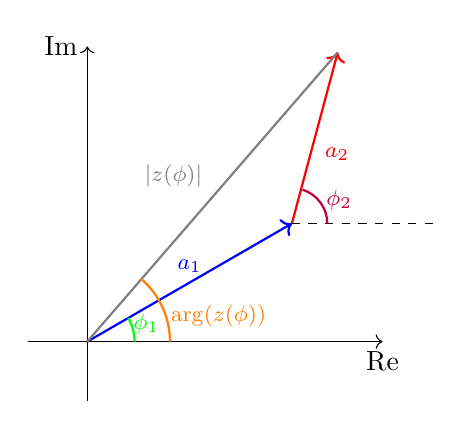
\begin{tikzpicture}[scale=1.5]
    % Define known parameters
    \def\aone{2}      % Magnitude of a1
    \def\phiOne{30}   % Angle phi1 in degrees
    \def\atwo{1.5}    % Magnitude of a2
    \def\phiTwo{45}   % Angle phi2 in degrees
    \def\phiExtend{27.5} % Additional angle to extend arc

    % Compute coordinates
    \pgfmathsetmacro{\Ax}{\aone * cos(\phiOne)}
    \pgfmathsetmacro{\Ay}{\aone * sin(\phiOne)}
    \pgfmathsetmacro{\Bx}{\Ax + \atwo * cos(\phiOne + \phiTwo)}
    \pgfmathsetmacro{\By}{\Ay + \atwo * sin(\phiOne + \phiTwo)}

    % Compute Phi(z(phi)) angle
    \pgfmathsetmacro{\PhiZ}{atan2(\By, \Bx)}

    % Define coordinates
    \coordinate (O) at (0,0);
    \coordinate (A1) at (\Ax,\Ay);
    \coordinate (A2) at (\Bx,\By);

    % Draw Axes
    \draw[->] (-0.5,0) -- (2.5,0) node[below] {$\mathrm{Re}$};
    \draw[->] (0,-0.5) -- (0,2.5) node[left] {$\mathrm{Im}$};

    % Draw vectors
    \draw[->,blue,thick] (O) -- (A1) node[midway, above  ] {\footnotesize $a_1$};
    \draw[->,red,thick] (A1) -- (A2) node[midway, below right] {\footnotesize $a_2$};

    % Draw resultant vector |z(phi)|
    \draw[gray, thick] (O) -- (A2) node[midway, above left] {\footnotesize $|z(\phi)|$};

    % Horizontal dotted line at end of a1
    \draw[dashed] (A1) --++ (1.2,0);

    % Draw angles φ1, φ2, and Φ(z(φ))
    \draw[green,thick] (0.4,0) arc (0:\phiOne:0.4);
    \node[green] at (0.5,0.15) {\footnotesize $\phi_1$};

    %  Arc (φ2) 
    \draw[purple,thick] ($(A1)+(0.3,0)$) arc (0:\phiTwo+\phiExtend:0.3);
    \node[purple] at ($(A1)+(0.4,0.2)$) {\footnotesize $\phi_2$};

    % Draw arc for Phi(z(phi))
    \draw[orange,thick] (0.7,0) arc (0:\PhiZ:0.7);
    \node[orange] at ({1.1*cos(\PhiZ/2)}, {1*sin(\PhiZ/2) - 0.20}) {\footnotesize $\;\;\;\;\arg(z(\phi))$};

    % Title
    %\node at (0,2.7) {\footnotesize %Visualization of $z(\phi) = a_1 %e^{i\phi_1} + a_2 e^{i\phi_2}$};

\end{tikzpicture}
\caption{Geometric representation of~$z(\phi)=z(\phi_1,\phi_2)$.\label{fig:viewz}}
\end{figure}


The canonical (Haar)  probability measure on the torus is
\begin{equation}\label{haar}
d\mu=\frac1{(2\pi)^n} d\phi_1\dots d\phi_n.
\end{equation}
\iffalse
For any~$r\geq0$, define the probability
\begin{align}
P(r;a_1,\dots,a_n)&:=\text{prob} ( |z(\phi_1,\dots,\phi_n)|\leq r )\nonumber\\
&=\int_{|z|\leq r} d\mu.
\end{align}


Suppose, we are given a sequence $a_k,\,k=1,\dots,n$ of real numbers. We associate with a point $(\phi_1,\dots,\phi_n)\in \T$ the following complex number: $z=\sum a_ke^{i\phi_k}$. This number describes the position of the end-point of a multi-link with link lengths $a_k$, and angle $\phi_k$ between $k$-th and $(k+1)$-th links.
\fi
Let~$W_n(r)=W_n(r;a_1,\dots,a_n)$ denote the probability 
that~$|z|\leq r$, where $z=z(\phi_1,\dots,\phi_n)$. Thus,
\begin{align}\label{eq:W_n(r)}   W_n(r) =
\int_{ |z|\leq r }d\mu
\end{align}
is the ``volume'' of all the angles in the $n$-dimensional
 torus
yielding~$|z|=|\sum _{k=1}^n a_ke^{i\phi_k}|\leq r$.


For small values of~$n$, $W_n(r)$ can be computed explicitly using geometric arguments. 
The next example demonstrates this. 

 \begin{example}
Consider the case~$n=2$. Fix~$a_1,a_2>0$. 
We compute~$W_2(r)=W_2(r;a_1,a_2)$ for any~$0\leq r\leq a_1+a_2$. 
To do so, we first determine 
all the angles~$0\leq\phi_1,\;\phi_2< 2\pi$ such that~$|z|=|a_1e^{i\phi_1}+a_2e^{i\phi_2}|\leq r$.
Since the calculation of~$W_2(r)$ is 
  invariant with respect to rotations, we  may assume that~$\phi_1=0$ (see Fig.~\ref{fig:two_d}).
  %%
  \begin{figure}[H]
 \begin{center}
%%%%%%%%%%%%%%%%%%%%%%%[width=12cm,height=12cm]
  \includegraphics[scale=0.6]{W222.eps}
  \caption{Plotting $z=a_1e^{i\phi_1}+a_2e^{i\phi_2}$, with~$\phi_1=0$, in the complex plane.}
  \label{fig:two_d}
%%%%%%%%%%%%%%%%%%%%%%%%%%
\end{center}
\end{figure}
%%%%%%%%%%%%%%%%%%%%%%%%%%%%
  We have
\begin{align*}
    |z|^2&=\big(a_1+a_2\cos(\phi_2)\big)^2+\big(a_2\sin(\phi_2)\big)^2\\
    &=a_1^2+2a_1a_2\cos(\phi_2)+a_2^2 .
 \end{align*}
   Let  
\begin{align}\label{eq:def_q}
    q(r;a_1,a_2):=\frac{r^2-(a_1^2+a_2^2)}{2a_1a_2}.
\end{align}
Then~$|z|^2\leq r^2$ iff
\begin{align*}
    \cos(\phi_2)\leq q ,
\end{align*}
that is, iff 
\begin{align*}
    \arccos (q) \leq\phi_2\leq 2\pi-\arccos(q).
\end{align*}
 Eq.~\eqref{eq:W_n(r)} now gives 
\begin{align}\label{eq:W_2(r)}
    W_2(r)&=\frac{1}{(2\pi)^2}\int_0^{2\pi}d\phi_1\int_{\arccos(q)}^{2\pi-\arccos(q)}d\phi_2\nonumber\\
    &=\frac{1}{2\pi}\big(2\pi-2\arccos( q) \big)\nonumber\\
    &=1-\frac{\arccos(q)}{\pi}.
\end{align}
Note that~$ W_2(r)\in[0,1]  $, as expected.  If~$r=a_1+a_2$  then~$q=1$  and~\eqref{eq:W_2(r)} gives~$W_2(r)=1$.
If~$r=|a_1-a_2|$  then~$q=-1$  and~\eqref{eq:W_2(r)} gives~$W_2(r)=0$ (see Fig.~\ref{fig:two_d}). 

%%%%%%%%%%%%%%
\begin{comment}
    %%%%%%%%%%%%%%
\noindent For~$\ell=1$,~$W_2(r)=1$. This case corresponds to $r\geq|z|$ as expected. 

For~$\ell=-1$,~$W_2(r)=0$. This case corresponds to~$r\leq |a_1-a_2|$, and indeed in this case we expect that~$W_2(r)=0$.  Substituting~\eqref{eq:W_2(r)} in~\eqref{mean} we have
\begin{align*}
    \Omega&=\sum_{i=1}^3\Big(1-\frac{\arccos\big(\ell(a_i;a_{i-1},a_{i+1})\big)}{\pi}\Big)\lambda_i\\
    &=\sum_{i=1}^3\lambda_i-\frac{1}{\pi}\sum_{i=1}^3\lambda_i\arccos\big(\ell(a_i;a_{i-1},a_{i+1})\big).
\end{align*}
Here, if~$i=1$,~$a_{i-1}=a_3$, if~$i=3$,~$a_{i+1}=a_{1}$. Assume
\begin{align*}
    a_1>a_2+a_3,
\end{align*}
then~$a_3<a_1-a_2$,~$a_2<a_1-a_3$, and we know that in this case
\begin{align*}
    W_2(a_1)=1,\;W_2(a_2)=W_2(a_3)=0,
\end{align*}
so~$\Omega=\lambda_1$.

\end{comment}
%%%%%%%%%%%%%%%%%%%%%%%%%%%%%%
\end{example}


The BBW formula   asserts  that \begin{equation}\label{BWW}
W_n(r;a_1,\dots,a_n)=r\int_0^\infty J_1(r\rho)\prod_{k=1}^n J_0(|a_k|\rho)d\rho,
\end{equation}
where $J_0,\,J_1$ are Bessel functions. Note that this
reduces the computation of the $n$-dimensional integral for~$W_n$ in~\eqref{eq:W_n(r)}
to a one-dimensional integral. 

%Note also  that it is {\em a priori} clear that $W_n(r;a_1,\dots,a_n)$ depends only on $r$ and $|a_1|,\dots,|a_n|$ because the set $\{\phi \in(\R/2\pi\Z)^n \suchthat |\sum a_ke^{i\phi_k}|\leq r\}$ is equal to the set
%$\{\phi \in(\R/2\pi\Z)^n \suchthat \left |\sum |a_k|e^{i(\phi_k+\arg( a_k))}\right |\leq r\}$, and the measure of the latter set  does not depend on $(\arg ( a_1),\dots,\arg (a_n))$.
For the sake of completeness, we include a self-contained
proof of~\eqref{BWW}
 in the Appendix.

 %%%%%%%%%%%%%
\subsection{Solution of the mean motion problem}
%%%%%%%%%%%%%%
Returning to Problem~\ref{prob:mean_motion}, 
  we say that the $\lambda_k$s in~\eqref{eq:rotating}
  are
  \emph{non-resonant}
  if there  are no non-trivial relations of the form 
  \be\label{eq:non_rse}
  \sum_{k=1}^n  \lambda_k \ell_k=0, \text{ where every }
\ell_k \text{ is an  integer}.
\ee
 Hermann Weyl \cite{Weyl_meanmotion} proved that under this condition the mean motion~$\Omega$ in~\eqref{eq:def_omeha}   exists, and satisfies
  \begin{equation}\label{mean}
\Omega=\sum_{k=1}^n \lambda_k V_k ,
\end{equation}
where
\be\label{eq:vks}
V_k : =W_{n-1}(a_k;a_1,\dots,a_{k-1},a_{k+1},\dots,a_n).
\ee
%{\bf need to check this}
%%%%
Furthermore,
the  $V_k$s  are non-negative, and $\sum_{k=1}^n V_k=1$~\cite{Weyl_meanmotion}.
In particular, if~$\lambda_k>0$ for all~$k$ then~$\Omega>0$, and if   all the~$\lambda_k$s are equal to a common value~$\lambda$ then Eq.~\eqref{mean} gives
\[ \Omega=\sum_{k=1}^n \lambda V_k=\lambda.
\]


Thus, the mean motion~$\Omega$ is a weighted  average of  the angular velocities $\lambda_k$.
The weight~$V_k$
corresponding to~$\lambda_k$
is  the ``volume''  of the set of points~$(\phi_1,\dots,\phi_{k-1},\phi_{k},\dots,\phi_n)$
in an~$(n-1)$-dimensional torus
such that~$   | {\displaystyle
\sum _{   %{\ell=1}, %\atop
%{
\ell \not = k}  }%^n
a_\ell e^{i\phi_\ell} |\leq |a_k|$.

\begin{example}
    Consider the case~$n=2$, that is,
    \[
    z(t)=a_1 e^{i(\lambda_1 t+ \mu_1) } +a_2 e^{ i(\lambda_2 t+ \mu_2) },
    \]
    and assume that~$|a_1|>|a_2|$. In this case, $a_2 e^{i(\lambda_2 t+ \mu_2) }$ is a ``small perturbation'' added to~$a_1 e^{i(\lambda_1 t+ \mu_1) }$.
  Eq.~\eqref{mean} gives~$\Omega=\lambda_1 V_1+\lambda_2 V_2$, where~$V_1$ is the
  probability that~$|a_2e^{i \phi}|\leq a_1$, that is,~$V_1=1$ (and similarly~$V_2=0$). Thus, in this case~$\Omega=\lambda_1$. 
  %%%%%%%%%%%%%
\end{example}

 
 Note that combining
 Eqs.~\eqref{mean}, \eqref{eq:vks},
 and the BBW-formula
 yields
 a closed-form  expression for the mean motion~$\Omega$
 in terms of  integrals of  Bessel functions.

\begin{example}
     Consider the case~$n=3$, $a_1= 1$,
     $a_2 =2.5$, $a_3=3$, $\lambda_1=\sqrt{2}$,
     $\lambda_2=3 $,~$\lambda_3=\sqrt{3}$
      and~$\mu_i=0$, $i=1,2,3$, so 
\begin{align*}
    z(t)=  e^{i \sqrt{2} t }+2.5 e^{i 3 t }+3  e^{i  \sqrt{3} t }.
\end{align*}
Then
\begin{align*}
    \Omega &= \sum_{i=1}^3 \lambda_i V_i\\
    &= \sqrt{2} W_2(1; 2.5,3)+3 W_2(2.5; 1,3)+\sqrt{3} W_2(3; 1,2.5)\\
    &= \sqrt{2}   \int_0^\infty J_1( \rho) 
    J_0( 2.5 \rho)J_0( 3 \rho)d\rho\\
    &+ 7.5   \int_0^\infty J_1( 2.5 \rho) 
    J_0(  \rho)J_0( 3 \rho)d\rho\\
    &+3\sqrt{3}   \int_0^\infty J_1( 3 \rho) 
    J_0(  \rho)J_0( 2.5 \rho)d\rho.
\end{align*}
Numerical integration  using Matlab gives
\[
\Omega=2.0614
\]
(to 4-digit accuracy). Fig.~\ref{fig:bessel}
 shows the value~$\frac{\arg(z(T)) }{T}$ as a function of~$T$, and it may be seen that this indeed converges to~$\Omega$ as~$T\to\infty$. 
%%%%%%%%%%%%%%%%%%%%%%
\end{example}

\begin{figure}[t]
\centering
\includegraphics[scale=0.6]{omri_plot_bessel.eps}
\caption{Plotting~$\frac{\arg(z(T)) }{T}$ as a function of~$T$. \label{fig:bessel}}
\end{figure}
 


\begin{remark}
    The BBW formula is a solution to a ``static'' problem of determining a ``volume'' of angles in the torus that satisfies a certain  inequality. The mean motion problem is ``dynamic'',  as it considers the asymptotic behaviour of the time-dependent function~$z(t)$. For the sake of completeness, we give an informal explanation on how these two problems are related. 
Since~$z(t)=|z(t)|e^{i\Phi(t)}$, we have~$\Phi(t)=\imag(\log(z(t)))$, so 
\begin{align*}
    \dot \Phi(t) &= \imag (\frac{\dot z(t)}{z(t)})\\
    &=\imag (  \frac{\sum a_k\lambda_k   i e^{i(\lambda_k t +\mu_k)}}{\sum a_k e^{ i(\lambda_k t+\mu_k)}}  ) \\
    &=\real (  \frac{\sum a_k\lambda_k     e^{i(\lambda_k t +\mu_k)}}{\sum a_k e^{ i(\lambda_k t+\mu_k)}}  ) .
\end{align*}
This implies that we can view~$\dot\Phi(t)$ as a mapping from~$(\lambda_1 t,\dots,\lambda_n t)\in\T$
to~$\R$. Now, 
\begin{align}\label{eq:intg_rih}
\Omega&=\lim_{t\to\infty}\frac {\Phi(t)-\Phi(0)}{t}\nonumber\\
&=\lim_{t\to\infty}
\frac1{t}\int_0^t \dot \Phi(s)ds,
\end{align}
  and the non-resonance condition implies that we can calculate this  integral 
using  a ``static'' integral over the torus. 
%%%%%%%%%%%%%
%%%%%%%%%%%%
\end{remark}

\begin{remark}
   %%%%%%%%%%%%%%%%%
Eq.~\eqref{mean} holds even if condition~\eqref{eq:non_rse} is relaxed to  the following {\em almost non-resonancy} condition: there  are no non-trivial relations of the form $\sum_{\ell=1}^n \lambda_k \ell_k=0$, where
the~$\ell_k$s are integers, and $\sum_{k=1}^n \ell_k=0$. If~$\lambda_1=\dots=\lambda_n$
then the non-resonance condition fails, but the almost non-resonance condition holds. 
 %%%%%%%%%%%%%%%%%
\end{remark}

\begin{comment}
    The next example is about the BBW formula for $n=1$.
\begin{example}
    Consider the  case~$n=1$. Then~$z(\phi_1)=a_1 e^{i\phi_1}$, so
\begin{equation}\label{Wr}
        W(r)=\int_{|z|\leq r} d \mu
    = \begin{cases} 1,\text{ if } |a_1|\leq r,\\
        0,\text{ otherwise}.
        \end{cases}
    \end{equation}
Eq.~\eqref{BWW} gives
    $W(r)=r\int_0^\infty J_1(r\rho)J_0(a_1\rho)d\rho$  and this agrees with \eqref{Wr} according to a well-known formula \cite{watson} 13$\cdot$48, p. 420. The formula
\begin{equation}
a\int_0^\infty J_1(ax)J_0(bx)dx= \begin{cases} 1,\text{ if } |a|\leq |b|,\\
        0,\text{ otherwise}.
        \end{cases}
\end{equation}
can be proved directly: Indeed, from the Plancherel theorem \cite{stein_fourier} and the definition of the Bessel functions it follows that the (two-dimensional) Fourier transform of $f_a(x):=J_1(ax)$ and $g_b(x):=J_0(bx)$ is $\mathcal{F}f_a(\xi)=|\frac{\xi}{a}|1_{B_2}(\frac{\xi}{a})$, and $\mathcal{F}g_b(\xi)$ is the uniform probability  measure $d\mu(\frac{\xi}{b})$ on the circle of radius $b$. Therefore, $\int_0^\infty J_1(ax)J_0(bx)dx=\int_{\R^2}|\frac{\xi}{a}|1_{B_2}(\frac{\xi}{a})d\mu(\frac{\xi}{b})$. The last integral equals 0 if $|a|>|b|$ and $\frac1{a}$, if $|a|\leq b$.
\end{example}
In case $n=2$ there  also exists an elementary, but quite nontrivial, formula \cite{Weyl_meanmotion} for $W(a_1;a_2,a_3)$.

\end{comment}

\begin{remark}
Writing~\eqref{eq:rotating}  as
\[
z(t)   =\sum_{k=1}^n (a_k e^{i \mu_k} ) e^{i \lambda_k t  } ,
\]
and noting that~$\Omega$ does not depend on the~$\mu_k$s 
implies that we can actually assume that
the~$a_k$s in~\eqref{eq:rotating}  
are complex numbers,
and the formula for~$\Omega$ will depend
only on  the absolute values of the~$a_k$s. 
\end{remark}
 %%%%%%%%
\section{Main result}\label{sec:density}
%%%%%%%%%%%%%%%%%%%%%%%%%%

If the spectrum of~$A $ in~\eqref{eq:lin_cont_sys} is real then it is well-known (see, e.g., \cite[Theorem~6-8]{athans_falb})  that~$N(T)\leq n-1$ for any~$T > 0$. We consider the    case where  all the eigenvalues of~$A$ are purely imaginary. 
 
\begin{assumption}\label{assump:dominanat}
The dimension~$n$ is even and the 
eigenvalues of~$A\in\R^{n\times n}$ are 
\[
i\lambda_1, -i\lambda_1 ,\dots, i\lambda_{n/2}, -i\lambda_{n/2}, 
\]
where all the~$\lambda_k$s are real. 
\end{assumption}

\begin{comment}
    To state our main result we introduce more notation. Every eigenvalue of~$A$ with real part~$\nu$ has the form 
\[
\nu + i \eta,  
\]
with~$\eta\in \R\setminus\{0\}$,
and since~$A$ is real, $\nu - i \eta $ is also an eigenvalue of~$A$. 

Suppose that the linear system is controllable, and all the eigenvalues of the matrix $A$ with the maximal real part $\nu$ are not real. Consider the imaginary parts of these eigenvalues. They are encountered in pairs $\{\nu+i\lambda,\nu-i\lambda\}$. We can assume that $A=\oplus_{\mu\in\Spec A} A_\mu$, where $A_\mu$ is a Jordan cell, corresponding to the eigenvalue $\mu$. Choose one value $\mu_k=\nu_k+i\lambda_k$
 from each such pair $\{+i\lambda_k,-i\lambda_k\}$ and the corresponding eigenvector $v_k$.  Define  complex matrices  $\mathfrak{A}_{\mu_k}={A}_{\mu_k}$ and $\mathfrak{A}=\oplus_k\mathfrak{A}_{\mu_k}$
 with eigenvalues $\mu_k$, and eigenvectors $v_k$, and with the same structure of the Jordan cells as that of $A$.

\end{comment}

We can now state our main result. 

%%%%%%%%%%%%%%%%%%%%%%%%%%%%%%%%%
\begin{theorem}\label{thm:main}
%%%%%%%%%%%%%%%%%%%%%%%%%%%%%%%%
Suppose that~$A$ satisfies Assumption~\ref{assump:dominanat} and that the pair~$(A,b) $ is controllable. 
%
 Then, for   generic vectors~$p,b\in\R^{n}\setminus\{0\}$
 there exists~$c>0$ such that 
   for any~$T$ large enough  the number of zeros of the switching function~$m$ in~\eqref{eq:abst_m} on the interval~$[0,T]$ satisfies
   \[
   N(T)\geq c T+o(T).
   \]
 %%%%%%%%%%%%%%%%%%%%%%%%%%%%%%%%%%%%%%
\end{theorem}

The proof of this result, given below, can actually be used to
provide a closed-form
expression for~$c$ in terms of a  solution to 
the mean motion problem. 

\begin{IEEEproof}
%%%%
We may assume that there exists a non-singular matrix~$H\in\R^{n\times n}$ such that~$A=H^{-1}\diag(B_1,\dots,B_{n/2})H$, with
\[
B_i:=\begin{bmatrix} 0& \lambda_i\\-\lambda_i &0 \end{bmatrix}.
\]
%%%
The switching function~\eqref{eq:abst_m}  
becomes 
\begin{align*} 
m(t) &= p^\top  H^{-1} \diag(\exp(B_1 t),\dots,\exp(B_{n/2}t)) H b\\
&=  \sum_{k=1}^{n/2}  c_k \cos(\lambda_k t)+d_k \sin(\lambda_k t),
\end{align*}
where~$c_k,d_k\in\R$   depend on  the 
entries     of~$b$, $p$, and~$H$. Thus, 
\begin{align*} 
m(t) &= \real( \sum_{k=1}^{n/2}  c_k e^{i \lambda_k t}+
d_k e^{i(    \lambda_k t -(\pi/2) )}  )
\\
&=  \real(  \sum_{k=1}^{n/2}   a_k  e^{i \lambda_k t}   ) ,
\end{align*}
with~$a_k:=c_k+d_ke^{-i\pi/2}=c_k-id_k$. 
Define 
\[
z(t):= \sum_{k=1}^{n/2}   a_k  e^{i \lambda_k t} .
\]
 Every time~$t_i\geq 0 $ such that~$ \arg(z(t_i)) = \pi/2$ or~$\arg(z(t_i)) =3  \pi/2  $
is a zero of the swicthing function~$m(t)$. Consider the asymptotic
behavior of~$\arg(z(t))$ on the interval~$ [0,T]$, with~$T$  large.  
The solution of the mean motion problem implies that
\[\
\Omega : = \lim_{T\to\infty}  \frac{ \arg(z(T))-\arg(z(0))} {T} 
\]
exists and satisfies~\eqref{mean}. Thus, for~$T$ large enough  the number of zeros of~$m$ on the interval~$[0,T]$
is bounded from below by
\[
\frac{|\Omega|}{\pi}T+o(T) , 
\]
and this completes the proof of Theorem~\ref{thm:main}. 
%%%%%%%%%%%%%%
%%%%%%%%%%%%%
\end{IEEEproof}


\iffalse
\subsection{Conjectures}If we deal with a linear control system $$
\dot x=Ax+Bu,\,x\in V,\,|u|\leq1
$$
we automatically get a canonical decomposition of the phase space $V=V_0+V'$, where both subspaces $V_0,\,V'$ are $A$-invariant, and if $\lambda,\lambda'$ are eigenvalues of $A$ on $V_0$, while $\mu,\mu'$ are eigenvalues of $A$ on $V'$, then $\lambda-\lambda'\in i\R$ is purely imaginary, while $\mu-\mu'\in\R$ is real.
\fi
\iffalse
Here, we turn to the following problem. Suppose, that the number of switching point is infinite in the infinite interval of time. Consider a finite interval $[0,t]$, and let the number  of switching points in the interval be $N(t)$. If $N(t)\to\infty$ as $t\to\infty$ then $N(t)/t$ has a limit $\nu$ as $t\to\infty$, and we would like to describe this limit explicitly in terms of the parameters $A,\,b$ of the linear system $\dot x=Ax+bu$.
\fi

 
\begin{example}
    %%%%%
Consider  the case where~$n=4$,
\[
A=\begin{bmatrix}
    0 & \zeta_1 & 0 &0 \\
    -\zeta_1 &0 &0 &0\\
    0&0&0&\zeta_2\\
    0 & 0& -\zeta_2 &0 
\end{bmatrix},
\]
with~$\zeta_1,\zeta_2\not =0$,  
$\zeta_1>\zeta_2$,
and~$b=\begin{bmatrix}
   0& 1&0&1
\end{bmatrix}^\top$. 
Thus,~$A$ has distinct
purely imaginary eigenvalues:~$i\zeta_1,-i\zeta_1,i\zeta_2,-i\zeta_2$. 
A calculation shows that  
\begin{align*}
\det \begin{bmatrix}
    b& Ab & A^2b&A^3b
\end{bmatrix} &=\zeta_1 \zeta_2 (\zeta_1^2-\zeta_2^2)^2\\&\not=0,
\end{align*}
so the pair~$(A,b)$ is controllable. 
System~\eqref{eq:lin_cont_sys} becomes
\begin{align}\label{oscillators}
\ddot x_1 &+\zeta_1^2 x_1=\zeta_1 u,\nonumber\\
\ddot x_3&+\zeta_2^2 x_3=\zeta_2 u. \nonumber
\end{align}
This describes  the motion of two  linear oscillators (e.g., springs)
coupled  by a common  forcing term~$u(t) $ (and in the optimal control problem we assume that~$|u(t)|\leq 1$ for all~$t$).
%%%%%%%%%%%%%%%%%%
In this case, 
\begin{align*}
  %%
  m(t)&=p^\top  e^{-At} b \\
    &= -p_1\sin(\zeta_1 t) -p_3\sin(\zeta_2 t) 
     +p_2 \cos(\zeta_1 t) +p_4 \cos(\zeta_2 t) .
 %%%%   
\end{align*}
%%%
This can    be expressed as
\begin{align*}
     m(t)&= \real ( - p_1 e^{i(\zeta_1  t-(\pi/2))}  -p_3 e^{i(\zeta_2 t-(\pi/2))}\\&+p_2  e^{i \zeta_1 t}+p_4
  e^{i \zeta_2 t} )   \\
  &=\real (a_1 e^{i\zeta_1 t} +  a_2 e^{i\zeta_2 t}
  ) ,
%%
\end{align*}
 %%
 with~$a_1:=-p_1 e^{-i\pi/2}+p_2$ and~$a_2:=-p_3 e^{-i\pi/2} +p_4 $.    
 %%%
%%%%
\end{example}


For low values of~$n$  it is possible to give more accurate bounds
for~$N(T)$ and show that they agree with the asymptotic lower bound in Theorem~\ref{thm:main}.
The next result  demonstrates this. 


\begin{proposition}\label{prop:two_oscillators}
   Consider the case where
    \begin{align*} 
       m(t)=\real(a_1e^{i\lambda_1 t}+a_2e^{i\lambda_2 t}), 
    \end{align*}
    with~$a_1,a_2\in\R\setminus\{0\}$,
  and  assume, without loss of generality, that
    \[
    \lambda_1>\lambda_2.
    \]
  If~$a_1>a_2$ then
     \begin{align} \label{eq:a1la2}
        \frac{\lambda_1}{\pi}T\leq N(T)\leq\frac{\lambda_1}{\pi}T+1,\text{ for all }T>0.
    \end{align}
If~$a_1<a_2$ then 
 \begin{align} \label{eq:seclow}
        \frac{\lambda_2}{\pi}T\leq N(T)\leq\frac{\lambda_1}{\pi}T,\text{ for all }T>0.
    \end{align}
    \end{proposition}
%%%
 %%
    \begin{IEEEproof}
A time~$t_i$ is zero of~$m(t)$ iff
\[
 \cos(\lambda_2 t_i) =-\frac{a_1}{a_2} \cos(\lambda_1 t_i).
\]
Suppose that~$a_1>a_2$. 
Fix an integer~$\ell\geq 0$, and consider the time interval
\[
L_1:=[\frac{2\pi\ell}{\lambda_1},  \frac{2\pi\ell}{\lambda_1}+\frac{\pi}{\lambda_1}].
\]
On this time interval,~$-\frac{a_1}{a_2}\cos(\lambda_1 t)$ is monotonic, and attains all the values from~$-a_1/a_2$ to~$a_1/ a_2$ and since~$a_1>a_2$, we conclude that it intersects~$\cos(\lambda_2t)$ at least once. Also, since~$\lambda_1>\lambda_2$ there is exactly one such intersection, so $m(t)$ has   a single  zero on~$L_1$. A similar argument shows that~$m(t)$ has exactly one zero on 
\[
L_2:=[   \frac{2\pi\ell}{\lambda_1}+\frac{\pi}{\lambda_1}, \frac{2\pi(\ell+1)}{\lambda_1}  ].
\]
Thus, there are two zeros of~$m(t)$ in  every period of~$   \cos(\lambda_1 t)$. This proves~\eqref{eq:a1la2}.

Now consider the case~$a_1<a_2$.  The upper bound on~$N(T)$ in~\eqref{eq:seclow} is obtained arguing similarly as above, but noting that now~$|a_1/a_2|<1$. 
To derive the lower  bound, 
fix an integer~$\ell\geq 0$, and consider the time interval
\[
\tilde L_1:=[\frac{2\pi\ell}{\lambda_2},  \frac{2\pi\ell}{\lambda_2}+\frac{\pi}{\lambda_2}].
\]
On this time interval,~$ \cos(\lambda_2 t)$ is monotonic, and attains all the values in the range~$[-1,1] $.  Since~$-\frac{a_1}{a_2}\cos(\lambda_1t)$ takes values inside the interval~$(-1,1)$, there is at least one zero of~$m(t)$ in~$\tilde L_1$.  Arguing similarly as above on the interval
\[
\tilde L_2:=[  \frac{2\pi\ell}{\lambda_2}+\frac{\pi}{\lambda_2},
\frac{2\pi(\ell+1)}{\lambda_2}  ] 
\]
gives the lower bound on~$N(T)$ in~\eqref{eq:seclow}. 
    \end{IEEEproof} 


 
Not that  Proposition~\ref{prop:two_oscillators} implies that 
    \begin{align*} 
        \frac{\lambda_2 }{\pi}T\leq N(T),  \text{ for all } T>0,
    \end{align*}
  and this agrees with the asymptotic 
  linear bound  in Theorem~\ref{thm:main}.
 

%%%%%%%%%%%%%%
%%%%%%%%%%%%%%
\begin{comment}
    Our problem is to understand the limit behavior of the number $N(T)$ of zeroes of the switching function in the interval $[0,T]$ as $T\to\infty$. This is related to the rotation of the complex number $z(t)=\sum a_ke^{i(\lambda_k t+\mu_k)}$ as $t$ runs over the interval $[0,T]$. If $z(t)\neq0$ for $t\in [0,T]$ and makes $m$ full rounds as $t$ runs over the interval $[0,T]$, then there are  at least $2m$ zeroes of $m(t)$ in this interval.

The relation of the mean angular velocity of $z(t)$ with the $N(T)$ is important, but we can get results in a more straightforward way, by studying  $\int_0^T |m(t)| dt$. Here, the central result (which goes back to \cite{gleich_verteilung}) is as follows (\cite{GOvs}):
\begin{theorem}\label{modulus}
Suppose that~$A:\R^n\to \R^n$ is a  diagonalizable  matrix with a purely imaginary spectrum, $p,\,b\in\R^n$. Then, the ergodic mean (wrt time) \begin{equation}\label{central}
\lim_{T\to\infty}\frac{\int_0^T |m(t)| dt}{T}=\lim_{T\to\infty}\frac{\int_0^T |pe^{tA}b| dt}{T}
\end{equation}  does exist, and is equal to the space average $$\int_{\mathcal T}|p\mathbf{t}b| d\mathbf{t},$$
where ${\mathcal T}$ is the closure of the one-parameter subgroup $e^{tA}$, and $d\mathbf{t}$ is the unique probabilistic Haar measure \eqref{haar} on ${\mathcal T}$.
\end{theorem}
Another relevant, but much more simple result is that there is a universal constant $C>0$ such that \begin{equation}\label{estimate}
\left|\int_I m(t) dt\right|\leq C,
\end{equation} where $I$  is an arbitrary interval of time. This follows from the similar estimates for $\left|\int_I \cos(t) dt\right|$.  Note, that the basic difference between expressions in \eqref{central} and \eqref{estimate} are the different positions of the modulus sign.

By comparison Theorem \ref{modulus} and the bound \eqref{estimate} we can easily get the following result on the distribution of the switching points:
\begin{theorem}\label{lower}
The number $N(T)$ of zeroes of the switching function in the interval $[0,T]$ has the lower bound $N(T)\geq CT$, where $C$ is a positive constant, as $T\to\infty$.
\end{theorem}
\begin{proof}Indeed, it follows from  Theorem \ref{modulus} that $\int_I |m(t)| dt\geq c|I|$, where $c>0$, $|I|$ is the length of   a sufficiently long interval $I$. On the other hand, according to \eqref{estimate}, the  integral of the switching function $\int_I m(t) dt=O(1)$. Therefore, as soon as $c|I|$ is greater that the constant $C$ from the bound \eqref{estimate} we conclude that the interval $I$ contains a zero of the switching function $m(t)$. For otherwise, the function $t\mapsto|m(t)|$ is equal either $t\mapsto m(t)$ or $t\mapsto -m(t)$ for all $t\in I$. This means, in particular, that  $N(T)$ grows linearly with $T$.
\end{proof}


\end{comment}


\begin{comment}
    \begin{example}
Note, that the result of Theorem \ref{lower} is well-known for classical two-dimensional control system of a linear oscillator \cite{athans_falb}: $$
\left[\begin{array}{c}\dot x_1\\\dot x_2\end{array}\right] =\left[\begin{array}{cc}0&\omega\\-\omega &0\end{array}\right] \left[\begin{array}{c} x_1\\ x_2\end{array}\right] +\left[\begin{array}{c}0\\ u\end{array}\right],
$$
where the number of switchings $N(T)$ equals the integer part of $\frac{ |\omega|}{\pi} T$.%+\varepsilon,\text{ where %|\varepsilon|\leq1$.
\end{example}

\end{comment}


\begin{comment}
    These results can be extended to the case of non-diagonalizable $A$. The result of Theorem~\ref{lower} remains true. But the proof should be modified, since the switching function now takes the form
\begin{equation}\label{multiple}
 m(t)=\Re\sum p_k(t)e^{i\lambda_k t},
\end{equation}
where $p_k(t)$ is a polynomial. Suppose, $d$ is the maximal degree of all polynomials $p_k$. Then $ m_d(t):=\sum_{\deg p_k=d} t^d a_k e^{i\lambda_k t}$, where $a_k$ is the higher order coefficient of $p_k$, is  asymptotically the main part of the switching function. E.g., the $L_1$-norm of $m(t)-m_d(t)$ over the interval $[0,T]$ is of order $O(T^d)$, while the same norm of  $m_d(t)$ is greater than $cT^{d+1}$. This (lower) bound for $\Vert m_d(t)\Vert_{L_1}$  can be proved in the same way as in the proof of Theorem \ref{lower}, which corresponds exactly to the case $d=0$.

Indeed, $\int_0^T t^d|\sum a_ke^{i\lambda_k t}|dt=T^dv(T)-\int_0^T (dt^{d-1})v(t) dt$, where $v(t)=\int_0^t|\sum a_ke^{i\lambda_k s}|ds$. According to Theorem \ref{modulus} asymptotically $v(t)\thicksim ct$, where $c$ is a positive constant, and $t\to+\infty$. Therefore, asymptotically, as $t\to+\infty$ we have $\int_0^T t^d|\sum a_ke^{i\lambda_k t}|dt=T^d cT-\int_0^T (dt^{d-1})ct dt\sim\frac{cT^{d+1}}{d+1}$.


We conclude that $L_1$-norm of $m(t)$ over the interval $[0,T]$ is of exact order $c'T^{d+1}$: \begin{equation}\label{lowerd}
\Vert m\Vert_{L_1(0,T)}\geq c'T^{d+1},\, c'>0.
\end{equation}
This estimate again (exactly as in the case $d=0$) implies the linear growth oh $N(T)$.

\begin{comment} while the proof requires another facts from \cite{GOvs}, namely:
\begin{theorem}\label{modulus2}
Suppose $A=D+N:\R^n\to \R^n$ is a   matrix with a purely imaginary spectrum, where $D$ is diagonalizable, $N$ is nilpotent, $DN=ND$, $p,\,b\in\R^n$. Then,  there exists an invertible matrix function $F(T)$ such that  the limit $F_\infty:=\lim_{T\to\infty}F(T)$ exists, and the ergodic mean (wrt time) \begin{equation}\label{central2}
\lim_{T\to\infty}\frac{\int_0^T |pF(T)e^{tA}b| dt}{T}
\end{equation}  exists, and is equal to the space average $$\int_{{\T}\times[0,1]}|pe^{N\tau}\mathbf{t}F_\infty b| d\mathbf{t}d\tau,$$
where ${\T}$ is the closure of the one-parameter subgroup $e^{tA}$, and $d\mathbf{t}$ is the unique  Haar measure on ${\T}$ of mass 1.
\end{theorem}

\end{comment}


\begin{comment}

 \begin{theorem}\label{imaginary}
Suppose that the linear system is controllable, and all the eigenvalues of the matrix $A$ with the maximal real part  are not real. Then, for a generic $ p\in\R^n$ the number of roots of the function $t\mapsto p^\top e^{At}b$ in the interval $[0,T]$ of time is greater that $cT$. Here $c>0$ is a strictly positive constant, and $T>0$ is sufficiently large.
\end{theorem}
\begin{proof}
 This result gives a linear lower bound for the number of switching points for a control system $\dot x=-Ax+bu$, with the governing matrix $A$, since the switching function for the system  is $p^\top e^{At}b$.

This can be proved by a straightforward generalization of the proof of Theorem \ref{lower}. Indeed, consider the $L_1(0,T)$-norm of the function $g(t):=e^{-\nu t}f(t)$, where $\nu$ is the maximal real part of eigenvalues of $A$, and $f$ is the switching function. Then, if the ``dual vector'' $p$ has a non-zero component in the root space of $A^\top$, corresponding to an eigenvalue with the real part $\nu$,   the leading term in  the $L_1(0,T)$-norm of $g$ looks like $\int_0^T|\sum a_k(t)e^{i\mu t}|dt$, where $\mu$ runs over the imaginary parts of the eigenvalues with the real part $\nu$, and $a_k$ is a polynomial in $t$. This expression is studied in the proof of Theorem \ref{lower} and is shown to be greater than $ cT^{d+1},\, c>0,$ where $d$ is the maximal degree of polynomials $a_k$. On the other hand, the $\int_0^T\sum a_k(t)e^{i\mu t}dt=O(T^d)$. These two inequalities, pointing in opposite direction, are incompatible. This  shows that there is a zero of $g(t)$ in any sufficiently long interval of time.  Therefore, the number of zeroes of $g(t)$ in $(0,T)$ grows linearly with $T$. Since the zeroes of $g$ are exactly the same as that of the switching function $f$, we get the required lower bound on the amount of switches. \end{proof}

The above approach to distribution of switching points (zeroes of the switching function) does not lead, at least immediately, to an explicit formula for the density of  switching points. To get such a formula we should typically choose the real switching function of the form $m(t)=\Re\sum a_ke^{i(\lambda_k t+\mu_k)}$, and study instead the  complex switching function $M(t)=\sum a_ke^{i(\lambda_k t+\mu_k)}$. This function in general has no real roots, but the understanding of roots of $m(t)$ can be extracted from understanding of the {\it rotation} (angular velocity) of the 2-dimensional vector $M(t)$. The instants of $t$, when the curve $M(t)$ intersects the imaginary axis are exactly the zeroes of $m(t)$.

Therefore, computation of the asymptotic angular velocity of $M(t)$ is a key to finding the density of  switching points.

\end{comment} 

\begin{comment}
    Now, the main construction leading to computation of the (lower bound of) density of switching points is as follows:
Suppose that the linear system is controllable, and all the eigenvalues of the matrix $A$ with the maximal real part $\nu$ are not real. Consider the imaginary parts of these eigenvalues. They are encountered in pairs $\{\nu+i\lambda,\nu-i\lambda\}$. We can assume that $A=\oplus_{\mu\in\Spec A} A_\mu$, where $A_\mu$ is a Jordan cell, corresponding to the eigenvalue $\mu$. Choose one value $\mu_k=\nu_k+i\lambda_k$
 from each such pair $\{+i\lambda_k,-i\lambda_k\}$ and the corresponding eigenvector $v_k$.  Define  complex matrices  $\mathfrak{A}_{\mu_k}={A}_{\mu_k}$ and $\mathfrak{A}=\oplus_k\mathfrak{A}_{\mu_k}$
 with eigenvalues $\mu_k$, and eigenvectors $v_k$, and with the same structure of the Jordan cells as that of $A$.

Assume that $\mu_k$ are non-resonant.
\begin{theorem}\label{imaginary2}
 Then, for a generic $p\in\R^n$  the function $t\mapsto  p^\top e^{{\mathfrak A}t}b $ has the mean motion $\Omega$, and the number $N(T)$ of  roots of the function $t\mapsto p^\top e^{At}b=\Re p^\top e^{{\mathfrak A}t}b $   in the interval $[0,T]$ of time is no less than $\frac{|\Omega|}{\pi} T+o(T)$, if $T$ is large enough.
\end{theorem}
\begin{proof}
Indeed, for a generic $p$ the complex switching function $p^\top e^{{\mathfrak A}t}b$ is never zero, and in time $T$ the two-dimensional vector
$z(t):= p^\top e^{{\mathfrak A}t}b$ makes $\frac{|\Omega|}{2\pi}T+o(T)$ full rounds, and each round adds at least two intersection points, one with positive imaginary part, and one with negative imaginary part, of the curve $z(t)$ with the imaginary axis.
\end{proof}
Thus, if $n$ is the dimension of the minimal $A$-invariant space generated by root-vectors for non-real eigenvalues,  we get as many as ($2^{n/2}$) different explicit expressions for the lower bound of $\lim_{T\to\infty}\frac{N(T)}{T}$ in terms of Bessel functions. It is clear that the largest of these bounds corresponds to the choice of all $\lambda_k$ positive. Indeed, this follows from the mean motion formula $\Omega=\sum W_k\lambda_k$, where the coefficients $W_k$ are positive, and independent of ``angular frequencies'' $\lambda_j$.


Hypothetically, this bound $\frac{|\Omega|}{\pi}T$, where $\Omega=\sum W_k\lambda_k,\,\lambda_k\geq0$,  is exact, meaning that the limit
\begin{equation}\label{eq:density}
\lim_{T\to\infty}\frac{N(T)}{T}
\end{equation}
does exist and is equal to $\frac{|\Omega|}{\pi}.$
\iffalse
Note, that, at least theoretically, the $|\Omega|=|\Omega({\frak A})|$  depends on the choice of matrix $\frak A$, while the number $N(T)$ does not.

This provides us with some peculiar consequences. Note, that the mean motion $\Omega$ in Theorem \ref{imaginary2} depends, in principle, on the choice of the matrix $\frak A$, which, in turn, depends on the choice of sign $\pm$ in front of the imaginary part of eigenvalue $\mu_k=\nu_k\pm i\lambda_k$ of the matrix $A$.
\fi
\subsection{Mean motion in the case of multiple eigenvalues} We would like to extend our asymptotic computations to the case, when the governing matrix $A$ might have multiple eigenvalues. We already did this by studying the $L_1(0,T)$-norm of the switching function. Now we expound parallel arguments, based on the study of rotation of a complex vector. This amounts to the asymptotic behavior of the vector
\begin{equation}\label{m_m_motion}
z(t)=\sum a_k(t)e^{i(\lambda_k t+\mu_k)},
\end{equation}
where, unlike \eqref{rotating}, the coefficients $a_k=a_k(t)$ are not constants, but polynomials in $t$. The degrees of these polynomials reflects the sizes of the Jordan cells of the matrix $A$.

In fact, as in the proof of Theorem \ref{lower} the asymptotic study of the vector $z(t)$ of \eqref{m_m_motion} reduces to the case of the constant $a_k$. Indeed, if $c_k t^{d_k}$ is the higher degree term of the polynomial $a_k(t)$, then one can replace $z(t)$ with
\begin{equation}\label{m_m_motion2}
z(t)=\sum c_k t^{d_k}(t)e^{i(\lambda_k t+\mu_k)},
\end{equation} without changing  any related asymptotic value. We can further get rid completely of the polynomial part of $z(t)$ by keeping only $c_k t^{d_k}$ with maximal $d_k=D:=\max_j d_j$. This reduces vector $z(t)$ to $$t^{D}\sum c_k e^{i(\lambda_k t+\mu_k)},$$
which
has the same argument as $\sum c_k e^{i(\lambda_k t+\mu_k)},$ and can be studied exactly as the vector \eqref{rotating} studied by Hermann Weyl and other classics. In particular, the mean motion of the latter can be described by formulas of the preceding subsection.
%%%%%
\end{comment}

\section{Discussion}
%%%%
We studied  the number of switching  points~$N(T)$ in time-optimal controls of a single-input linear system on the interval~$[0,T]$. We showed that when  all the eigenvalues
of~$A$ are purely imaginary 
the number of switching points
is lower-bounded by~$c T$ for large~$T$.
By relating the question to the
solution of
the mean motion problem, we also provided 
 an explicit formula for~$c$ in terms of integrals  of Bessel functions.
To the best of our knowledge, this is the first connection between optimal control theory and the mean motion problem. 



An interesting question is whether the
bound can be strengthened to
\begin{equation}\label{asymp_eq2}
N(T)= \tilde c T+o(T), \text{ as } T\to\infty,
\end{equation}
with an  explicit positive parameter~$\tilde c$.
The relation to the mean motion problem suggests that~$\widetilde c=\frac{|\Omega|}{\pi}$, where~$\Omega=\sum \lambda_k V_k  $, and the probabilities $$V_k:=W_{n-1}(a_k;a_1,\dots,a_{k-1},a_{k+1},\dots,a_n)$$ are given by the BWW formula \eqref{BWW}.
Another natural research direction is to extend the analysis to the case where~$A$ has  a more general spectral structure.  


%%%%%%%%%%%%%%%%%%%%%%%%%%%%%%%%%%%%%%%%%%%%
 \section*{Appendix: proof of the BWW formula }
 %%%%%%%%%%%%%%%%%%%%%%%%%%%%%%%%%%%%%%%%%%%%
Let~$\xi:=\sum_{k=1}^n  a_ke^{i\phi_k}\in \C$.
Fix~$r>0$.
By definition,
\be\label{eq:bydef_W}
W_n(r)=\frac1{(2\pi)^n}\int_{\T} 1_{|\xi|\leq r}(\xi)  \prod_{k=1}^n d\phi_k . 
\ee
Writing
\begin{equation}
1_{|\xi|\leq r}(\xi)=1_{B^2}(\xi/r),
\end{equation}
and applying an inverse Fourier transform to~\eqref{eq:ind_func_B2} yields
\begin{align*}
1_{|\xi|\leq r}(\xi)&=1_{B^2}(\xi/r)\\&=\frac{1}{2\pi}\int_\C |\eta|^{-1} J_1(|\eta|)e^{i\Re  (\bar\eta \xi/r )} d\eta .
\end{align*}
%%%%%%
Defining the integration variable
  $\theta:=\eta/r$ gives
\begin{equation}
1_{|\xi|\leq r}(\xi)= \frac{r}{2\pi}\int_\C |\theta|^{-1} J_1(r|\theta|)e^{i\Re  (\bar\theta \xi )} d\theta.
\end{equation}
Substituting  this in~\eqref{eq:bydef_W} yields
%%%%%%%%%%%%%%%%%%%%%
\begin{align*}
%%%%%%%%%%%%%%%%
W_n(r)&=\frac{r}{ 2\pi }\int_{\T}  \int_\C |\theta|^{-1} J_1(r|\theta|)e^{i\Re  (\bar\theta \sum_{k=1}^n a_ke^{i\phi_k}  )} d\theta\\&\times \frac1{(2\pi)^n} \prod_{k=1}^n d\phi_k\\
%%%%%%
&= \frac{1}{ 2\pi }\frac{1}{(2\pi)^n}\int_{\T}  \int_\C |\theta|^{-1} J_1(r|\theta|)\\&\times
\left (  \prod_{k=1}^n e^{i\Re  (\bar\theta  a_k e^{i\phi_k}  )}d\phi_k\right)  d\theta  .
%%%%%%%%%%%%%%
\end{align*}
Write~$ \theta$ in the polar representation~$   \theta=\rho e^{i \alpha }$, where $\rho:=|\theta|$. Then
%%%%
\begin{align*}
 \frac1{2\pi}  \int_0^{2\pi } e^{i\Re  (\bar\theta  a_k e^{i\phi_k}  )}d\phi_k &=\frac1{2\pi}
  \int_0^{2\pi }  e^{i\Re  ( \rho a_k   e^{i(\phi_k-\alpha)}  )}d\phi_k\\
  &=\frac1{2\pi}  \int_0^{2\pi }  e^{i \rho \Re  (  a_k   e^{i \beta_k  }  )}d\beta_k\\
  &= \frac1{2\pi}  \int_0^{2\pi }  e^{i \rho   |a_k|  \cos(\beta_k)  }d\beta_k\\
  &= J_0(\rho |a_k|).
\end{align*}
%%%%
Thus,
\begin{align*}
W_n(r)
%%%%%%
&= \frac{1}{ 2\pi }   \int_\C |\theta|^{-1} J_1(r|\theta|)\left (  \prod_{k=1}^n J_0(|\theta| |a_k|)   \right)  d\theta  .
\end{align*}
 The integrand
 \[
 |\theta|^{-1} J_1(r|\theta|) \prod_{k=1}^n J_0(|\theta| |a_k|)
 \]
 is a radial function, and using known results on the integration of radial functions (see, e.g.,~\cite[Chapter~6]{real_analysis_stromberg})
gives
%%%%
\begin{align*}
W_n(r)
%%%%%%
&=  r \int_0^\infty  J_1(r \rho ) \left (  \prod_{k=1}^n  J_0(\rho |a_k|)    \right)  d\rho,
\end{align*}
and this completes the proof of the BWW formula .




%\bibliographystyle{IEEEtranS}
%\bibliography{omri}

% Generated by IEEEtranS.bst, version: 1.14 (2015/08/26)
\begin{thebibliography}{10}
\providecommand{\url}[1]{#1}
\csname url@samestyle\endcsname
\providecommand{\newblock}{\relax}
\providecommand{\bibinfo}[2]{#2}
\providecommand{\BIBentrySTDinterwordspacing}{\spaceskip=0pt\relax}
\providecommand{\BIBentryALTinterwordstretchfactor}{4}
\providecommand{\BIBentryALTinterwordspacing}{\spaceskip=\fontdimen2\font plus
\BIBentryALTinterwordstretchfactor\fontdimen3\font minus \fontdimen4\font\relax}
\providecommand{\BIBforeignlanguage}[2]{{%
\expandafter\ifx\csname l@#1\endcsname\relax
\typeout{** WARNING: IEEEtranS.bst: No hyphenation pattern has been}%
\typeout{** loaded for the language `#1'. Using the pattern for}%
\typeout{** the default language instead.}%
\else
\language=\csname l@#1\endcsname
\fi
#2}}
\providecommand{\BIBdecl}{\relax}
\BIBdecl

\bibitem{athans_falb}
M.~Athans and P.~L. Falb, \emph{Optimal Control: An Introduction to the Theory and Its Applications}.\hskip 1em plus 0.5em minus 0.4em\relax McGraw-Hill Book Company, 1966.

\bibitem{levinson_select}
J.~Nohel and H.~J. Sussmann, ``{Commentry on Minimax, Liapunov and Bang-Bang},'' in \emph{Selected Papers of Norman Levinson}, J.~A. Nohel and D.~H. Sattinger, Eds.\hskip 1em plus 0.5em minus 0.4em\relax Boston: Birkhauser, 1998, vol.~2, pp. 463--475.

\bibitem{SHARON_3_nilp}
Y.~Sharon and M.~Margaliot, ``Third-order nilpotency, nice reachability and asymptotic stability,'' \emph{J. Diff. Eqns.}, vol. 233, no.~1, pp. 136--150, 2007.

\bibitem{sontag_book_control_theory}
E.~D. Sontag, \emph{Mathematical Control Theory: Deterministic Finite Dimensional Systems}.\hskip 1em plus 0.5em minus 0.4em\relax New York, NY: Springer, 1998.

\bibitem{Four_intro}
E.~M. Stein and G.~Weiss, \emph{Introduction to Fourier Analysis on Euclidean Spaces}.\hskip 1em plus 0.5em minus 0.4em\relax Princeton, NJ: Princeton University Press, 1990.

\bibitem{real_analysis_stromberg}
K.~R. Stromberg, \emph{Introduction to Classical Real Analysis}.\hskip 1em plus 0.5em minus 0.4em\relax Belmont, CA: Wadsworth Inc., 1981.

\bibitem{suss_nice_reach}
H.~J. Sussmann, ``Reachability by means of nice controls,'' in \emph{Proc.\ 26th IEEE Conf. on Decision and Control}, vol.~26, 1987, pp. 1368--1373.

\bibitem{watson}
G.~N. Watson, \emph{A Treatise on the Theory of Bessel Functions}, 2nd~ed.\hskip 1em plus 0.5em minus 0.4em\relax Camebridge, UK: Cambridge University Press, 1980.

\bibitem{Weyl_meanmotion}
H.~Weyl, ``Mean motion,'' \emph{Amer. J Math.}, vol.~60, pp. 889--896, 1938.

\bibitem{Wintner-1933}
A.~Wintner, ``Upon a statistical method in the theory of diophantine approximations,'' \emph{Amer. J. Math.}, vol.~55, no.~1, pp. 309--331, 1933.

\end{thebibliography}

\end{document}



%%%%
\begin{comment}
 
  
%file omri_example_Bessel

 fun1=@(x)  besselj(1,x).*besselj(0,2.5*x).*besselj(0,3*x);
 
 fun2=@(x)  besselj(1,2.5*x).*besselj(0,x).*besselj(0,3*x);
 
 fun3=@(x)  besselj(1,3*x).*besselj(0,x).*besselj(0,2.5*x);

  
 i1=sqrt(2)*integral(fun1,0,Inf);
 i2=7.5*integral(fun2,0,Inf);
 i3=3*sqrt(3)*integral(fun3,0,Inf);

 total=i1+i2+i3

%%% now generate figure
hold off;
arr=[];
for t=0:.1:500   
    z=exp(i*sqrt(2)*t)+2.5*exp( i*3*t)+3*exp(i*sqrt(3)*t);
    arr=[arr angle(z)];
end

plot(0:.1:500,unwrap(arr)./(0:.1:500),'k')

grid on;
xlabel('$T$',Interpreter='latex',FontSize=16)


\end{comment}
